\section{Arquitectura y tecnologías} \label{sec:arq}
% explicarase a arquitectura empregada para alcanzar os obxectivos propostos.

    \subsection{Arquitectura del sistema}

        Se entiende que dada la variedad y versatilidad del sistema, no existe una arquitectura que pueda definirlo en su totalidad, ya que cada uno de los plugins tiene una forma de desarrollo y método de comunicación que depende directamente de su funcionalidad. Sin embargo, se puede decir que la arquitectura general del sistema está enfocada en un modelo \textit{Basado en componentes}.
        
        Este modelo de desarrollo de software enfatiza la descomposición del diseño en componentes funcionales o lógicos que se comuniquen mediante interfaces bien definidas. Esto permite alcanzar un mayor nivel de abstracción, ya que no se enfoca en las características específicas de cada componentes sino en el sistema en sí, y en la forma en que estos componentes son integrados.
        
        El \textit{desarrollo basado en componentes} ofrece algunas ventajas claras en este caso:
        \begin{itemize}
            \item \textbf{Facilidad de instalación y mantenibilidad} \\
            Tanto el software principal como los componentes son fácilmente reemplazables por nuevas versiones sin impacto en el resto del sistema.
            
            \item \textbf{Facilidad de desarrollo} \\
            Los componentes implementan interfaces bien definidas que proveen funcionalidades específicas, por lo que pueden ser desarrollados sin impactar otras partes del sistema.
            
            \item \textbf{Reusabilidad} \\
            Al definir componentes individuales, estos pueden ser reutilizados por diferentes aplicaciones y sistemas con características similares.
            
            \item \textbf{Aumento exponencial de funcionalidades} \\
            El desarrollo de componentes que interactúan entre sí permite que las nuevas funcionalidades puedan ser combinadas con las ya existentes, lo que posibilita satisfacer múltiples casos de uso con cada nueva integración.
        \end{itemize}

        \subsubsection{Componentes del sistema}
            En este apartado se detallan las diferentes partes que componen el sistema, así como la forma en la que se comunican entre ellas. En la figura \ref{fig:diagrama-de-componentes} se muestra un diagrama con los principales componentes, las interfaces de comunicación y los requisitos de cada uno de ellos.

            \begin{figure}[h!]
            \centering
                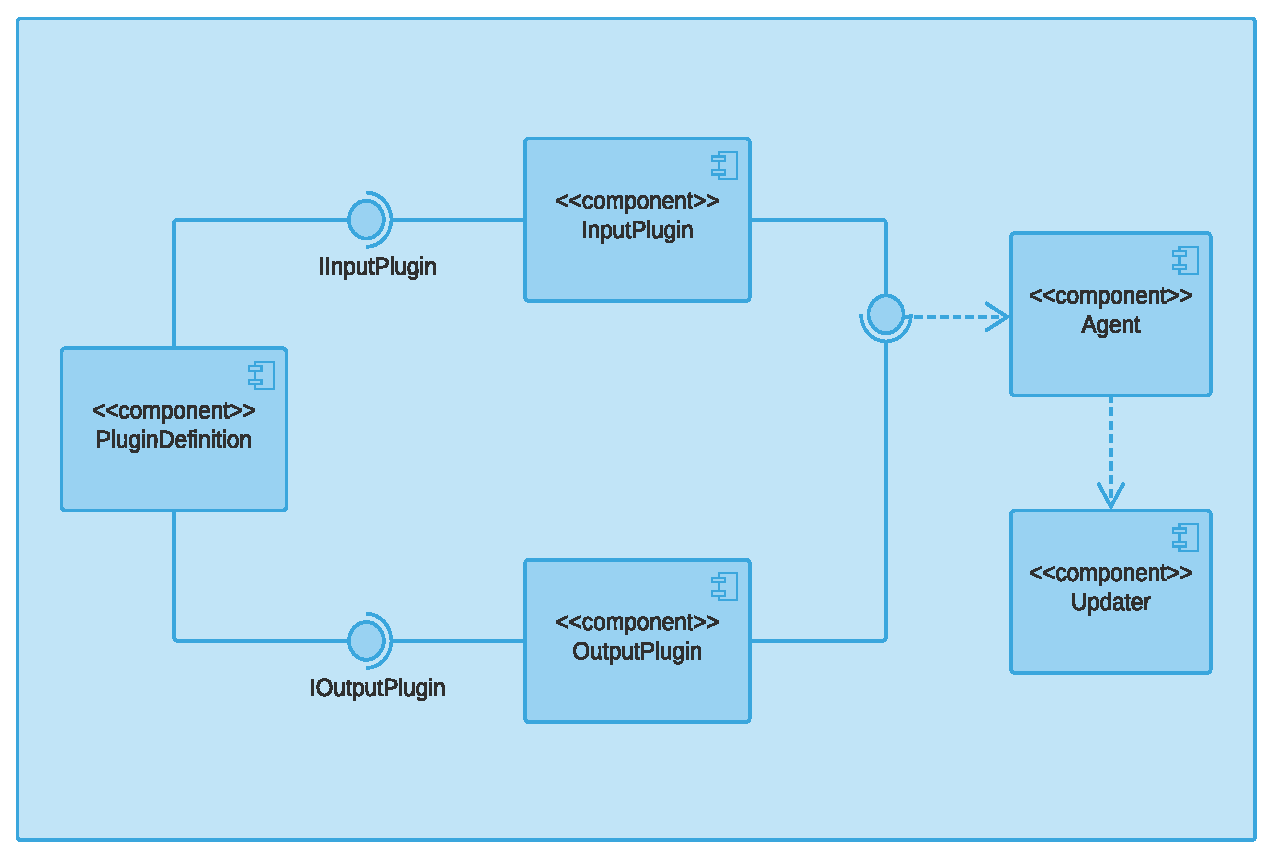
\includegraphics[scale=0.7]{diagrama-de-componentes.eps}
                \caption{Diagrama de componentes}
                \label{fig:diagrama-de-componentes}
            \end{figure}

        \subsubsection{Agente}
            El agente es el encargado de llevar a cabo la ejecución de los plugins con las opciones y configuraciones especificadas por el usuario, ya sea a través la línea de comandos o de un archivo de configuración. Además, será el responsable de ejecutar el proceso de actualización automática siempre que este haya sido configurado previamente. Está compuesto por un conjunto de clases, cada una de ellas realiza una tarea específica que le permite funcionar como un todo. En la figura \ref{fig:diagrama-de-arquitectura-winagent} se puede ver la estructura del agente.
            
            \begin{figure}[h!]
            \centering
                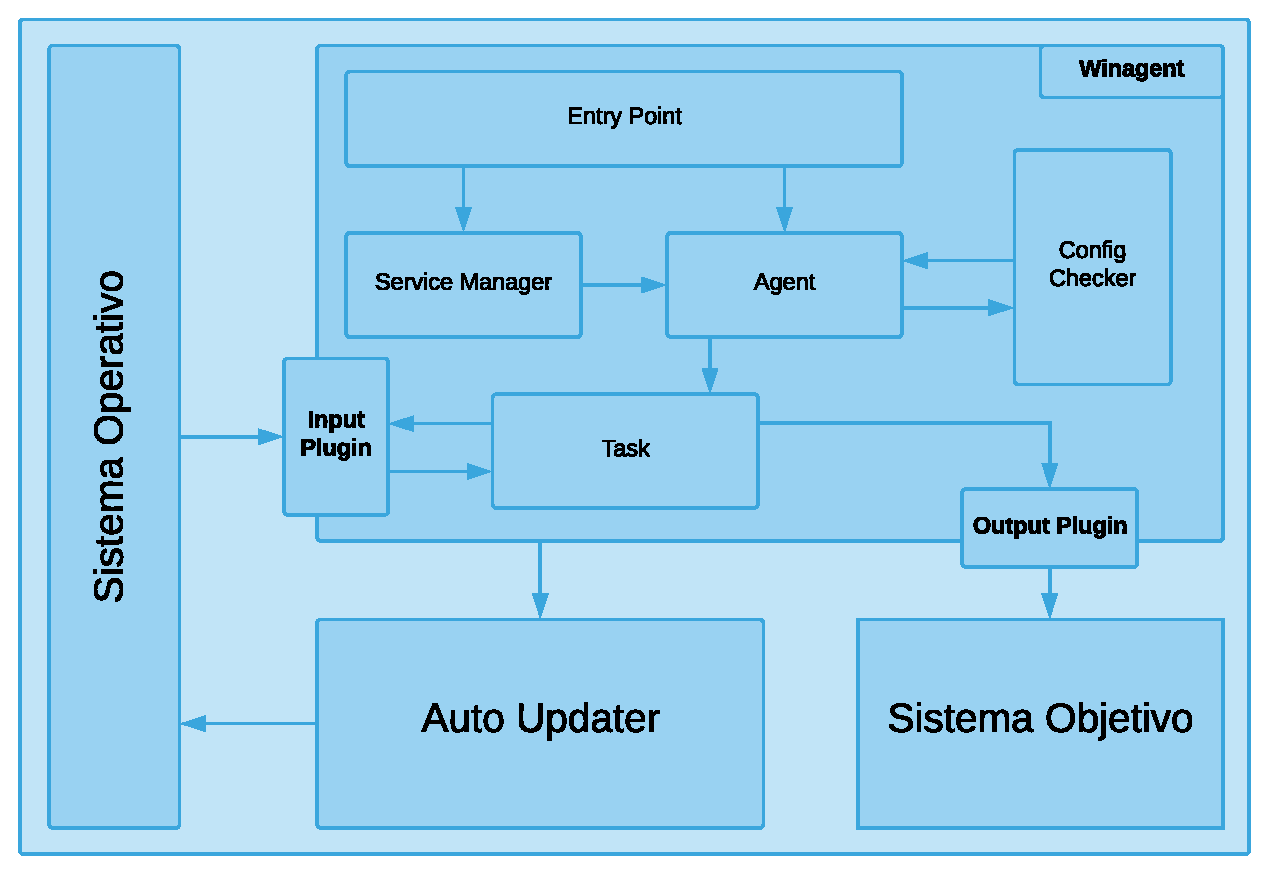
\includegraphics[scale=0.7]{diagrama-de-arquitectura-winagent.eps}
                \caption{Diagrama de arquitectura del sistema}
                \label{fig:diagrama-de-arquitectura-winagent}
            \end{figure}

            Las clases que componen el agente están separadas por su funcionalidad, interactúan entre sí y pueden ser utilizadas durante la ejecución o no, de acuerdo a las opciones y configuración establecidas. Entre las clases se pueden encontrar las encargadas de la inicialización del agente, las que gestionan el agente y sus configuraciones, y las que procesan y transmiten la información entre plugins.

            \begin{enumerate}
                \item Sistema de inicialización
                    \begin{itemize}
                        \item \textbf{Punto de entrada} \\
                        Sistema encargado de la inicialización del programa, determina si debe ser iniciado desde consola o como servicio en función del entorno desde el que sea ejecutado, y utiliza las opciones que le sean indicadas por el \textit{Analizador de comandos}.
                            
                        \item \textbf{Gestor de servicios} \\ 
                        Encargado de llevar a cabo la gestión del agente cuando se especifican opciones de control de servicio. Esto incluye instalación, desinstalación, ejecución y detención.
                            
                        \item \textbf{Analizador de comandos} \\ 
                        Es el sistema encargado de analizar sintácticamente las opciones introducidas por el usuario, las cuales varían para ejecuciones como servicio, consola con archivo de configuración predefinido y consola con opciones introducidas mediante linea de comandos.
                    \end{itemize}
                \item Planificador
                    \begin{itemize}
                        \item \textbf{Gestor de configuración} \\ 
                        Encargado de leer el archivo de configuración y proveer al \textit{Sistema de planificación} con la información definida previamente por el usuario.
                        
                        \item \textbf{Sistema de planificación} \\
                        En caso de que la orden sea ejecutada correctamente en el \textit{Sistema de funciones de configuración}, se envía un mensaje de confirmación específico dependiendo de la orden que haya sido recibida y procesada.
                    \end{itemize}
                \item Transmisor de información
                    \begin{itemize}
                        \item \textbf{Plugins de entrada} \\ 
                        Son los plugins encargados de recopilar información del sistema mediante el uso de librerías \textit{.NET}. Sirven esta información a los \textit{Plugins de salida}
                            
                        \item \textbf{Plugins de salida} \\
                        Son los plugins encargados de hacer llegar a la información recopilada por los \textit{Plugins de entrada} a los \textit{sistemas objetivos}. Dependiendo de la finalidad para la que hayan sido creados pueden utilizar diferentes métodos, desde mostrar datos por pantalla hasta enviarlos a un servidor remoto.
                        
                        \item \textbf{Tarea} \\
                        Es la funcionalidad que conecta los \textit{Plugins de entrada} con los \textit{Plugins de salida}, permitiendo que el primero reciba todos los parámetros configurados y agrupándolos como un único elemento capaz de ser configurado en el planificador.
                        
                    \end{itemize}
            \end{enumerate}

        \subsubsection{Actualizador automático}
            El sistema de actualización automática es el encargado de comprobar de forma periódica si las versiones instaladas son las últimas disponibles, esto incluye tanto el \textit{Agente} como los plugins y el propio actualizador.
        
            El sistema cliente es el encargado de realizar las peticiones al servidor. Su implementación en Android puede ser interpretada como el uso del patrón arquitectónico Modelo Vista Controlador, separando las vistas como los \textit{Layouts}, los controladores como las \textit{Actividades} y el modelo como las \textit{SharedPreferences} y los \textit{AsyncTasks}. En la figura \ref{fig:client_diagram} se puede ver la estructura del cliente.

            \begin{figure}[h!]
            \centering
                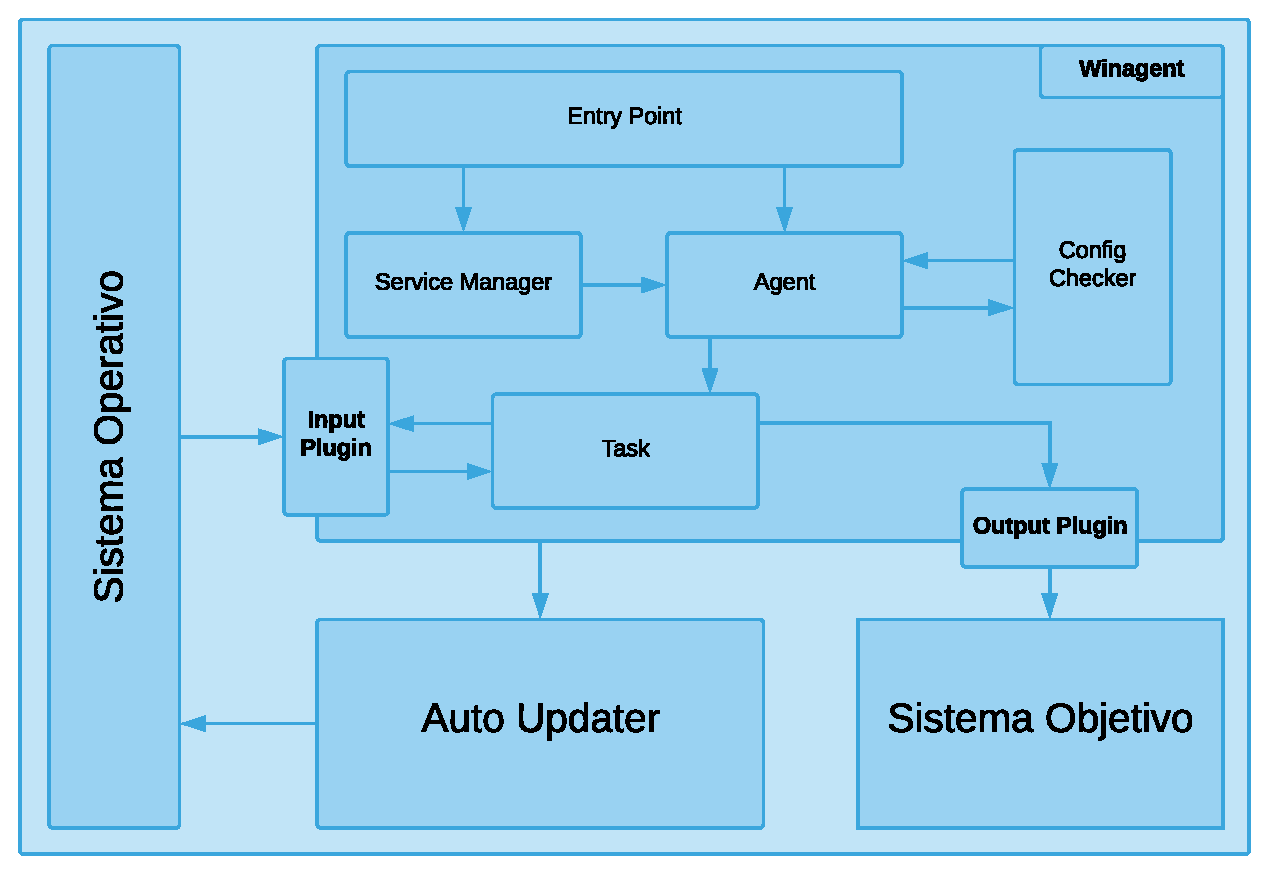
\includegraphics[scale=0.7]{diagrama-de-arquitectura-winagent.eps}
                \caption{Diagrama de arquitectura del actualizador}
                \label{fig:client_diagram}
            \end{figure}

            La arquitectura del cliente está dividida en tres componentes siguiendo el patrón de arquitectura MVC. Los \textit{Layouts} son renderizados desde el componente \textit{Actividades}, este es el encargado de gestionar la interacción con el usuario, haciendo uso de los componentes \textit{AsyncTask} siempre que sea necesario. El componente \textit{SharedPreferences} es utilizado para el almacenamiento de la configuración del cliente.

            A continuación se explica la función de cada uno de los subcomponentes del sistema:

            \begin{enumerate}
                \item Interfaz de usuario
                    \begin{itemize}
                        \item \textbf{\underline{Actividades}} \\
                            Realiza función de controlador, es el componente encargado de renderizar las vistas haciendo uso de los \textit{Resources} necesarios. Gestiona las entradas del usuario, y a partir de estas se comunica con el sistema servidor a través de los \textit{AsyncTask}.
                        \item \textbf{\underline{Resources}} \\ 
                            Es el componente que representa el conjunto de recursos necesarios para renderizar las vistas de forma correcta, y que estas a su vez, puedan ser gestionadas por las \textit{Actividades}.
                    \end{itemize}
                \item SharedPreferences
                    \begin{itemize}
                        \item \textbf{\underline{Editor}} \\ 
                            Permite almacenar elementos de forma sencilla como elementos clave-valor sin necesidad de utilizar una base de datos.
                        \item \textbf{\underline{Loader}} \\
                            Permiten recuperar los elementos clave-valor almacenados con el \textit{Editor}
                    \end{itemize}
                \item AsynckTask Servidor
                    \begin{itemize}
                        \item \textbf{\underline{Socket}} \\ 
                            Componente mediante el cual se recibe información desde el servidor y provoca cambios parciales en las vistas a detravés del \textit{Sistema rollback}.
                        \item \textbf{\underline{Sistema rollback}} \\
                            Realiza cambios parciales en las vistas a través de las \textit{Actividades}, bloqueando los elementos modificados y devolviéndolos a su estado original en caso de fallo.
                    \end{itemize}
                \item AsynckTask Cliente
                    \begin{itemize}
                        \item \textbf{\underline{Codificador DES}} \\
                            Utilizando la contraseña especificada por el usuario, aplica cifrado \textit{DES} a la información de control que luego es enviada al sistema servidor.
                        \item \textbf{\underline{Codificador Base64}} \\
                            Este componente es el encargado de cifrar en \textit{Base64} los datos obtenidos del \textit{Codificador DES} para que puedan ser enviados al sistema servidor a través del \textit{Socket}.
                        \item \textbf{\underline{Socket}} \\ 
                            Componente mediante el cual se envían los mensajes de control al sistema servidor en función de la entrada del usuario.
                    \end{itemize}
                    Componente que envía mensajes de control al sistema servidor, provoca cambios parciales en las vistas a través de la \textit{Actividad} desde la que es invocado
            \end{enumerate}

    % TODO: Estructure del "paquete" datos enviados

    \subsection{Tecnologías e integración de productos de terceros}
    % describiranse adecuadamente as tecnoloxías utilizadas para o desenvolvemento do traballo, así coma os diversos productos que non son da autoría do/da estudante, xustificando a súa utilización.
        \subsubsection{Microsoft Windows}
            Microsoft Windows es el nombre que recibe la familia de distribuciones basada en MS-DOS o Windows NT, desarrollada y comercializada por Microsoft Corporation. Estas estas distribuciones están disponibles para múltiples arquitecturas tales como x86, x86-64 o ARM, y hay opciones tanto para dispositivos de uso cotidiano como para servidores y sistemas de alta demanda. \cite{wikiwindows}
            
            Microsoft Windows, además, permite el uso de servicios \cite{wikiservicios}, programas que se ejecutan en segundo plano, proveyendo funcionalidades de forma transparente sin la necesidad de intervención por parte del usuario. Esta funcionalidad es perfecta para la utilización de un software que actúe como agente y se mantenga en ejecución permanentemente, proveyendo datos del equipo donde está instalado.
            
            \begin{itemize}
                \item \textbf{Windows 10} \\
                Dadas las similitudes de los sistemas \textit{Windows}, esta distribución pensada para la utilización de usuarios en entornos personales y laborales es la utilizada para el desarrollo del sistema que se propone. Permite llevar a cabo la creación del sistema de forma cómoda, sin necesidad de construir el entorno de desarrollo en un servidor administrado de forma remota.
                
                \item \textbf{Windows 2012 R2} \\
                Es la distribución instalada en la mayoría de servidores \textit{Windows} del CERN y sobre los que se desea utilizar el sistema que se desarrolla. Es utilizada para realizar pruebas periódicas que garanticen la compatibilidad con la plataforma de desarrollo; también se utiliza par llevar a cabo los procesos de construcción y publicación gestionados por \textit{gitlab-ci} en cada versión lanzada.
                
            \end{itemize}

        \subsubsection{Lenguaje C\#}
            Es un lenguaje de programación orientado a objetos diseñado y estandarizado por Microsoft como parte de \textit{.NET}, con el objetivo de permitir el desarrollo de aplicaciones y sistemas que fueran independientes de la arquitectura física y del sistema operativo sobre el que se ejecutaran. Es actualmente el lenguaje de programación más eficiente a la hora de trabajar con librerías de Windows por las facilidades que brinda para este tipo de desarrollos. \cite{csharp}

            \begin{itemize}
                \item \textbf{.NET Framework} \\
                Es una versión solo para \textit{Windows} de \textit{.NET}, la cual brinda interoperabilidad y cuenta con una gran librería de clases denominada \textit{Framework Class Library (FCL)}. Esta librería cubre diferentes aspectos como interfaces de usuario, bases de datos, conectividad, criptografía, desarrollo web, entre otros; permitiendo así llevar a cabo el desarrollo de aplicaciones de una forma sencilla sin tener un impacto directo en su calidad. \cite{netframework}
                
                \item \textbf{NuGet} \\
                Es un gestor de paquetes de código abierto que cuenta con una gran galería de librerías \textit{.NET} disponibles y que viene integrado por defecto en las últimas versiones de \textit{Visual Studio}. También provee las herramientas necesarias para la creación y utilización de estos paquetes, tanto en el período de desarrollo como en el período de construcción. \cite{nuget1} \cite{nuget2}

                \item \textbf{Newtonsoft} \\
                    Es la librería más popular para la gestión de información en formato JSON, de código abierto y alto rendimiento. Está disponible como paquete \textit{NuGet} y facilita la manipulación de datos mediante clases específicas para estructuras JSON. \cite{newtonsoft}

                \item \textbf{Commandline} \\
                    Esta librería ofrece una API concisa para manipular los argumentos recibidos en la aplicación mediante linea de comandos. Soporta el uso de verbos, opciones y switches. Provee además de algunas facilidades como un sistema de configuración de ayuda por defecto y una simple sintaxis de reporte de errores de cara al usuario. También disponible como paquete \textit{NuGet}. \cite{commandline1} \cite{commandline2}
                    
                \item \textbf{RabbitMQ} \\
                    Es una implementación para \textit{.NET} para el lado cliente de un sistema de colas \textit{AMQP}. Permite gestionar la conexión, estructura y parámetros de los mensajes enviados al servidor \textbf{RabbitMQ}. Implementa concurrencia, soporte a fallos y una amplia documentación. Es de código abierto y disponible como paquete \textit{NuGet}. \cite{rabbitmq}
                \item \textbf{ConsoleTableExt} \\
                    Una simple librería para estructurar la información mostrada a través de línea de comandos. Permite la imprimir datos JSON como una tabla, la cual dispone de diferentes formatos configurables. De código abieto y disponible como paquete \textit{NuGet}. \cite{consoletableext}
            \end{itemize}
            
        \subsubsection{Latex}
            Es un sistema de tipografía de alta calidad, incluye mecanismos diseñados para la creación de documentación científica y técnica por lo que se ha convertido en el estándar de facto a la hora de desarrollar esta tarea. Está concebido como software libre, y cuenta con múltiples librerías que añaden funcionalidades comúnmente necesarias para la creación de estos documentos. La documentación del desarrollo de este sistema está desarrollado con esta tecnología debido al conjunto de ventajas de estilo y edición que ofrece frente a otras tecnologías libres.

        \subsubsection{Git}
            Es un sistema de control versiones distribuido diseñado para controlar proyectos de cualquier tamaño con rapidez y eficacia. Es de código abierto y ofrece medios para guardar, analizar y revertir cambios realizados en versiones actuales y anteriores, además del control de ramas que permite mantener y trabajar en más de una versión de un proyecto de forma simultánea. Su uso en el desarrollo de este sistema viene justificado por las diferentes iteraciones/sprints que se llevan a cabo y el control de versiones necesario para su gestión.
            
        \subsubsection{PowerShell}
            Integrado en \textit{.NET}, PowerShell es un \textit{shell} de linea de comandos y un lenguaje de scripting de código abierto de gran utilidad para los administradores de sistemas, ya que tiene acceso a una gran cantidad de librerías que permiten gestionar equipos locales o remotos desde una consola de comandos. \cite{powershell}
        
        \subsubsection{CI/CD}
            \textit{Continuous integration} es la práctica que combina la compilación y la ejecución de pruebas automáticas (en caso aplicable) lo más a menudo posible, con el objetivo de detectar los fallos cuanto antes y evitar que una mayor cantidad de esfuerzo se vea comprometida.
            
            \textit{Continuous delivery} hace referencia la liberación de software en períodos cortos, reduciendo el coste, tiempo y riesgo de liberación de grandes versiones, apostando por unas más constantes e incrementales.
            
            \textit{Continuous deployment} consite en la automatización del proceso de puesta en producción. Para esto se utiliza el resultado del \textit{Continuous Delivery}, por lo que depende de unas pruebas automatizadas muy bien diseñadas. \cite{ci} \cite{cd} \cite{cicd}

    \subsection{Herramientas} 
        \subsubsection{Visual Studio 2017}
            Es un \textit{IDE} para Windows compatible con varios lenguajes de programación y, sin duda, la mejor opción disponible para programar en \textit{.NET}. \textit{Visual Studio}, además de otras plataformas de desarrollo, integra el gestor de paquetes \textit{NuGet} y soporta diferentes tipos de plugins creados por la comunidad, lo que facilita la creación de todo tipo de funcionalidades, desde aplicaciones de escritorio hasta webs, pasando por móviles, consolas y servicios. \cite{visualstudio} \cite{wikivisualstudio}

        \subsubsection{Visual Studio Code}
            Es una herramienta desarrollada por Microsoft que combina las simplicidad de un editor de texto con lo que necesitan los desarrolladores para su ciclo básico \textit{``edit-build-debug''}. Visual Studio Code provee soporte exhaustivo para la creación y depuración de código, además de un modelo extensible y una integración de bajo consumo de recursos con las herramientas existentes.

        \subsubsection{Overleaf}
            Es la principal plataforma de edición online para \textit{Latex} luego de haber integrado \textit{ShareLatex} incluyendo la mayoría de programas, micro paquetes y fuentes que son software libre. Ofrece soporte para múltiples idiomas, diferentes compiladores e integraciones con diferentes plataformas como \textit{Dropbox} y \textit{GitHub}.

        \subsubsection{Android Studio}
            Es el IDE (Integrated development environment) oficial para la creación aplicaciones Android. Ofrece herramientas para la edición de códigos de primer nivel, depuración, control de rendimiento y compilación instantánea. Provee de un emulador Android que permite comprobar el funcionamiento del código de forma rápida, y brinda un conjunto de opciones dinámicamente configurables en cuanto a tamaño, prestaciones y control de sensores. Posee integración condiferentes sitemas actuales y cuenta con soporte para librerías externas configurables para su compilación junto con la aplicación.

        \subsubsection{GitHub}
            Es una plataforma colaborativa de control de vesiones online basada en \textit{Git} y desarrollada por GitHub Inc. y que a día de hoy pertenece a Microsoft. Ofrece todas las funcionalidades de gestión de códigos que ofrece Git, así como sus propias características basadas en la web. Provee control de acceso y varias opciones colaborativas como el control de errores, petición de funcionalidades, gestión de tareas y wikis. La plataforma cuenta con un servicio de pago que permite la creación de repositorios privados, este servicio está disponible de forma gratuita junto a un conjunto de herramientas de desarrollo que la empresa ofrece en un paquete para estudiantes verificados.
            
        \subsubsection{GitLab}
            Es una una herramienta de código abierto que busca cubrir todo el ciclo de vida de un proceso de desarrollo. Ofrece todas las funcionalidades necesarias para un \textit{devops (desarrollo y operaciones)} como la gestión y planificación de proyectos, control de versiones, procesos de \textit{CI/CD}, monitorización y seguridad; además de disponer de integración con muchas otras plataformas. \cite{gitlab}

        \subsubsection{Lucidchart}
            Es una aplicación online enfocada a la creación de diagramas profesionales desde una interfaz web. Es una herramienta realmente cómoda a la hora de documentar proyectos grandes debido a lo sencillo y amigable de su entorno. Además, brinda integración con diferentes aplicaciones externas como Dropbox, Slack y Microsoft Office. 

        \subsubsection{Inkscape}
            Es un editor profesional de gráficos vectoriales disponible para Windows, Mac OS X y Linux. Es de código abierto y soporta una gran variedad de formatos, entre los que se incluye \textit{.eps}, el formato utilizado por latex. Además brinda una amplia variedad de herramientas para realizar trazado vectorial, manipulación de objetos y edición de textos.
